\documentclass{article}
\usepackage{a4wide}
\usepackage[T1]{fontenc}
\usepackage[utf8]{inputenc}
\usepackage[french]{babel}
\usepackage{empheq}
\usepackage{mathtools, bm}
\usepackage{amssymb, bm}
\usepackage{graphicx}
\usepackage{caption}
\usepackage{subcaption}
\usepackage{hyperref}
\usepackage{csvsimple}
\usepackage{float}

\title{\textbf{\Huge  Université Paris Saclay}\\ Rapport IAS}
\author{Guillaume Abadie, Jérôme Coquisart, Mathis Dupont, Martin Vitani}
\date{Année 2021}


\begin{document}
    \maketitle
    \tableofcontents
    \newpage

    \section{Introduction au problème}
    La ville de Chicago a un ratio de crimes, surtout sur les crimes violents, au dessus de la moyenne
    nationale des États-Unis.
    Les crimes dans la ville ont été collectés dès le début du 20ème siècle pour essayer de 
    comprendre pourquoi la ville était sujette à autant de violence.
    Le dataset correspond aux crimes commis entre 2001 et 2020, et contient environ 
    7 millions d'entrées.
    Tous les jours, la police de Chicago alimente la base de donnée avec les nouveaux crimes commis
    dans la ville. Seuls les meurtres ne sont pas comptabilisé dans la base de donnée.

    \section{Aperçu du dataset}
    \begin{figure}[H]
            \centering
	    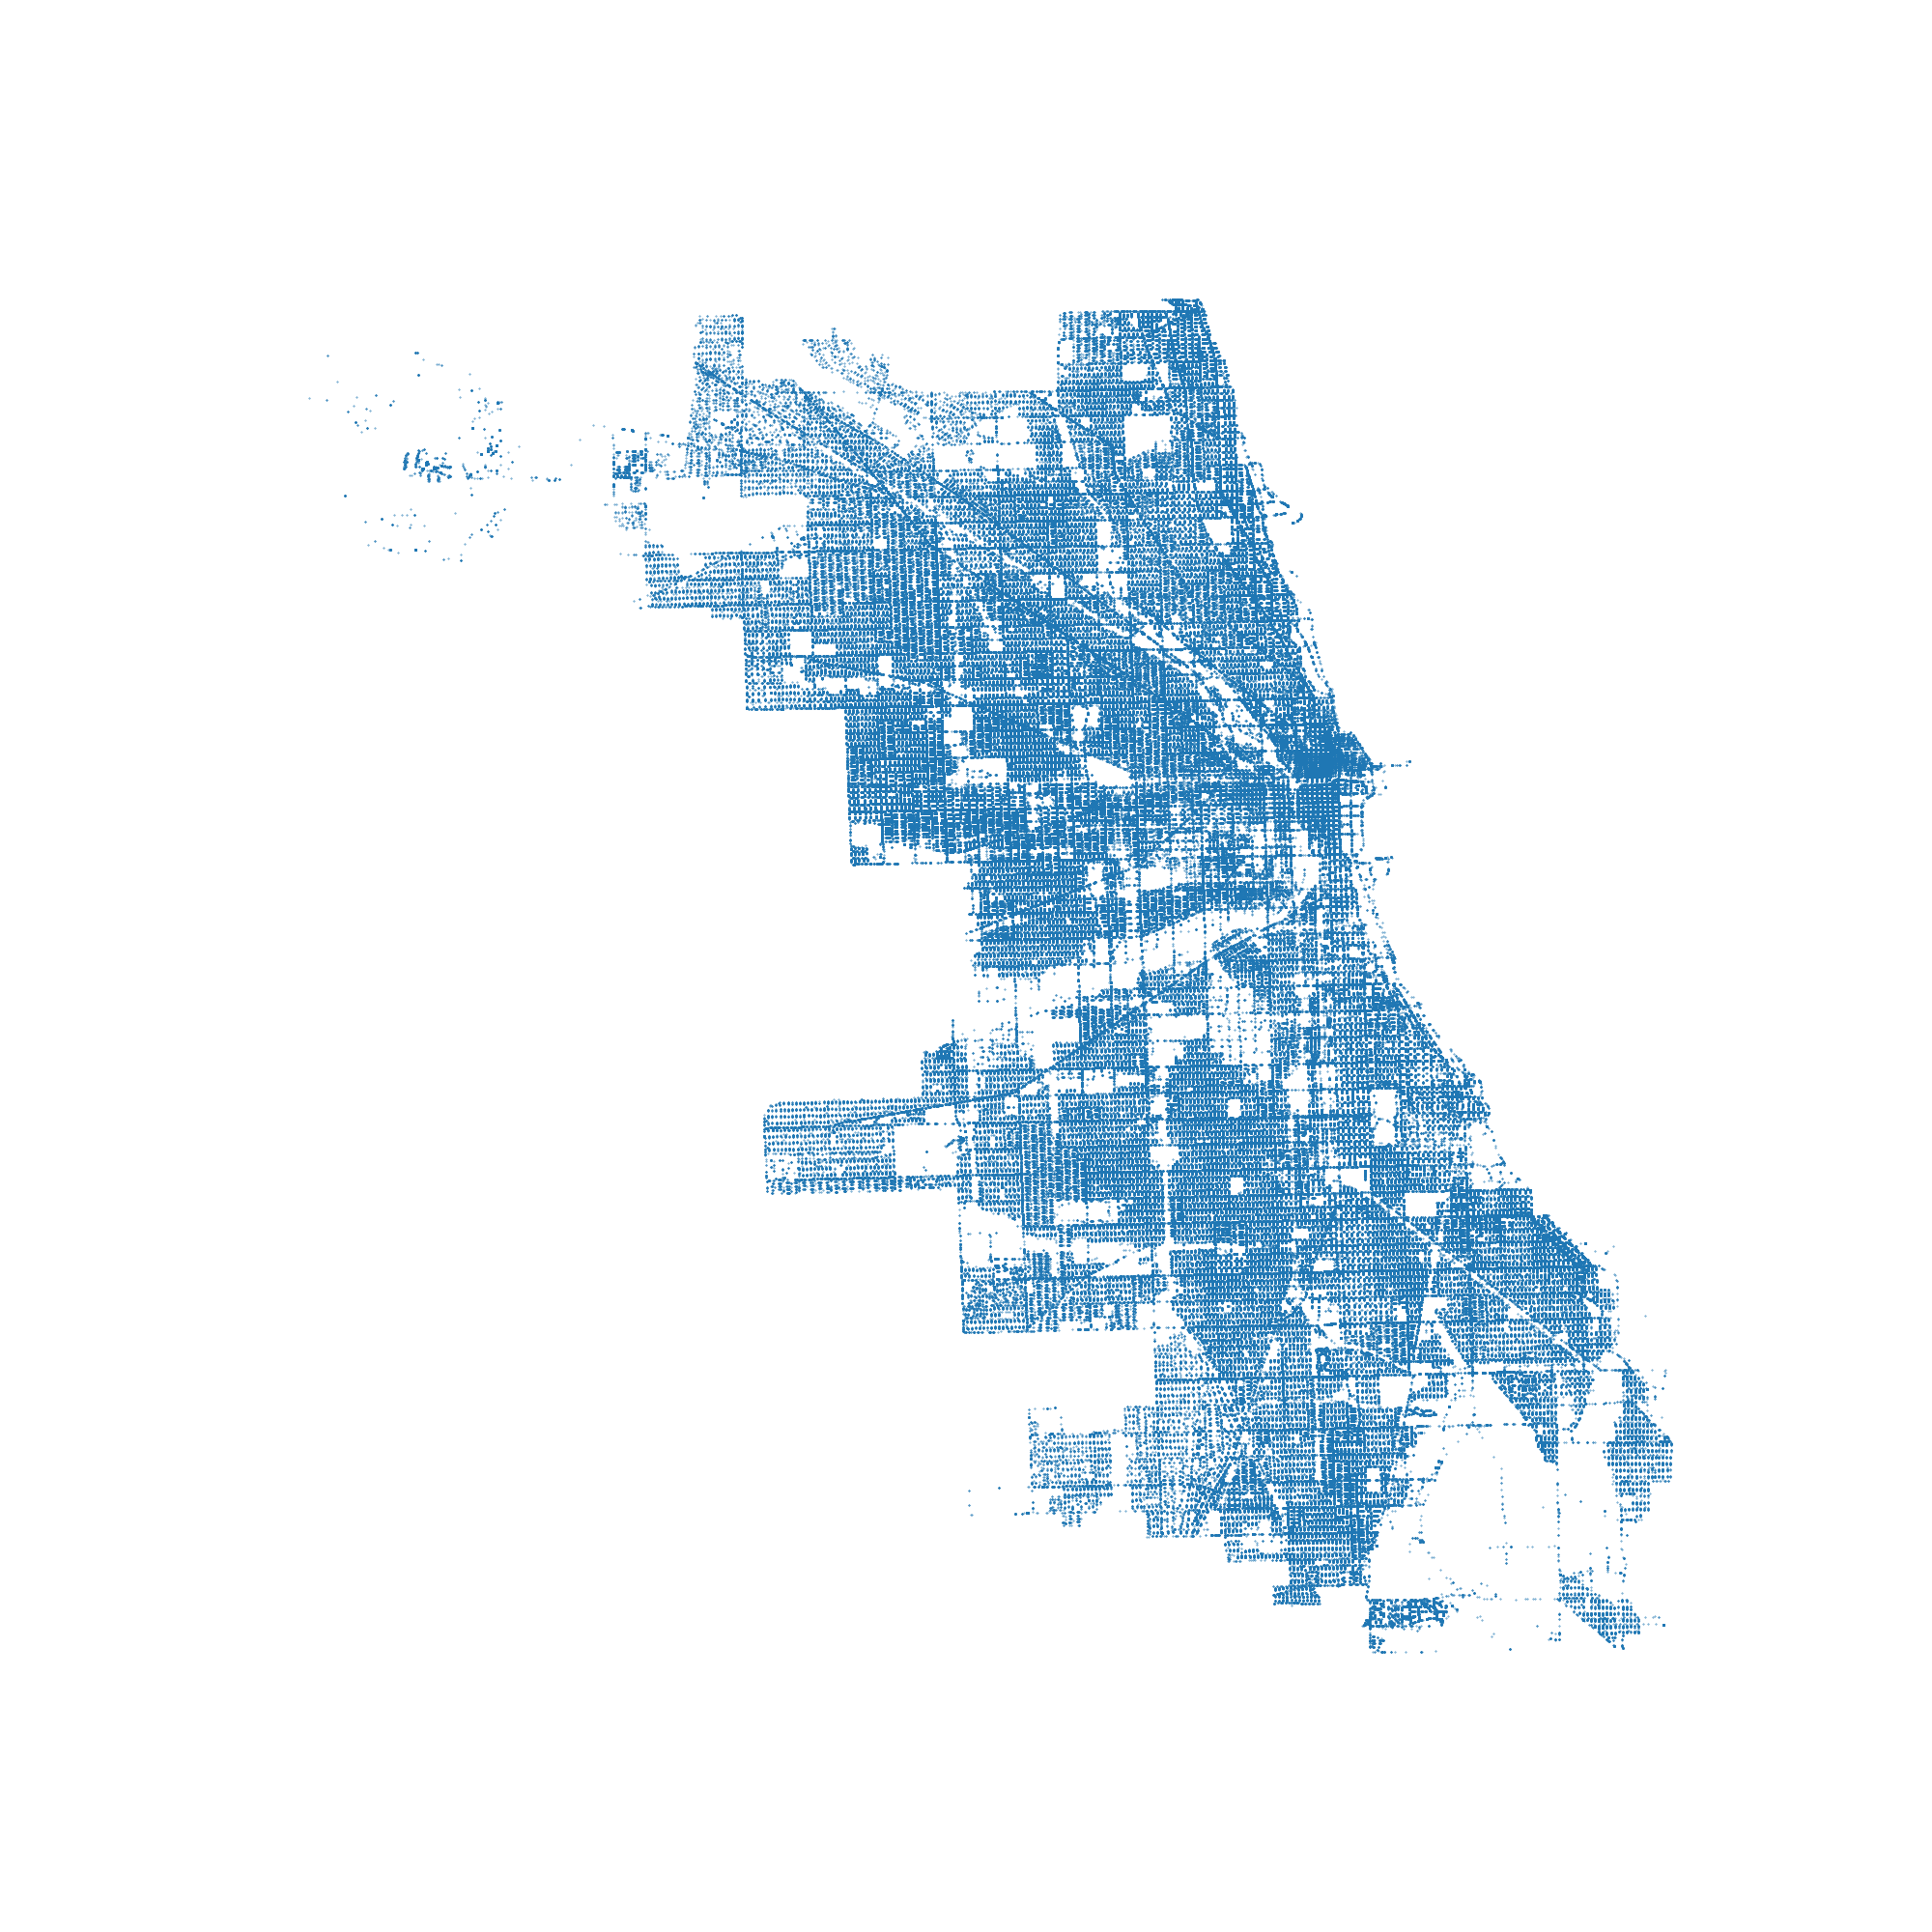
\includegraphics[scale=.2]{carte_chicago.png}
	    \caption{Carte représentant l'ensemble des crimes commis à Chicago}
    \end{figure}
    Sur cette carte, chaque point représente un crime.

    \section{Définition du problème}
    Notre problème sera le suivant. Il s'agira de déterminer si il y aura
    oui ou non une arrestation à la suite d'un crime. 
    Pour être plus précis, étant donné le lieu, la description et la date du crime, 
    il faudra dire si cela va mener à l'arrestation d'un suspect.
    C'est une tâche de classification
    binaire, en apprentissage supervisé.

    \section{Préprocessing}
    \begin{figure}[H]
            \centering
	    \includegraphics[scale=.2]{carte_densité.png}
    \end{figure}

    \section{Choix d'algorithme}

    \section{Comparaison des modèles}

    \section{Présentation des résultats}

    \section{Conclusion}

\end{document}
